% Created 2022-03-22 Tue 22:46
% Intended LaTeX compiler: pdflatex
\documentclass[11pt]{article}
\usepackage[utf8]{inputenc}
\usepackage[T1]{fontenc}
\usepackage{graphicx}
\usepackage{grffile}
\usepackage{longtable}
\usepackage{wrapfig}
\usepackage{rotating}
\usepackage[normalem]{ulem}
\usepackage{amsmath}
\usepackage{textcomp}
\usepackage{amssymb}
\usepackage{capt-of}
\usepackage{hyperref}
\usepackage[UTF8]{ctex}
\usepackage[vmargin={2.5cm,2.5cm},hmargin{2.5cm,2.5cm}]{geometry}
\usepackage{xcolor}
\usepackage{amsmath,bm}
\usepackage{newtxtext,newtxmath}

\newcommand{\quiz}[1]{\textcolor{red}{疑问:{#1}}}
\newcommand{\maxt}{\underset{t}{\mathrm{max}}}
\newcommand{\ut}{u(t)}
<<<<<<< HEAD
\newcommand{\ug}{u_\mathrm{g}}
=======
>>>>>>> 66231eb9c0179497516b0c0aebca8d85a4d84153
\newcommand{\usto}{(u_{\mathrm{st}})_{\mathrm{o}}}
\newcommand{\dut}{\dot{u}(t)}
\newcommand{\ddut}{\ddot{u}(t)}
\newcommand{\ddugt}{\ddot{u}_{\mathrm{g}}(t)}
\newcommand{\du}{\dot{u}}
\newcommand{\ddu}{\ddot{u}}
\newcommand{\uo}{u_\mathrm{o}}
\newcommand{\duo}{\ddot{u}_\mathrm{o}}
\newcommand{\dduo}{\ddot{u}_\mathrm{o}}
\newcommand{\dduto}{\ddot{u}^{\mathrm{t}}_\mathrm{o}}
\newcommand{\ddugo}{\ddot{u}_\mathrm{go}}
\newcommand{\uto}{{u}^{\mathrm{t}}_\mathrm{o}}
\newcommand{\ugo}{u_\mathrm{go}}
\newcommand{\uugt}{\ddot{u}_\mathrm{g}(t)}
\newcommand{\ddugt}{\ddot{u}_\mathrm{g}(t)}
\newcommand{\Tn}{T_\mathrm{n}}
\newcommand{\fn}{f_\mathrm{n}}
\newcommand{\omegan}{\omega_\mathrm{n}}
\newcommand{\omegann}{\omega^{2}_\mathrm{n}}
% \newcommand{\bmit}[1]{\bm{\mathit{#1}}} % 中译本用斜体
\newcommand{\bmit}[1]{\bm{\mathrm{#1}}}  % 原著用正体
\newcommand{\vm}{\bmit{m}}
\newcommand{\vddu}{\ddot{\bmit{u}}}
\newcommand{\vdu}{\dot{\bmit{u}}}
\newcommand{\vu}{\bmit{u}}
\newcommand{\vf}{\bmit{f}}
\newcommand{\vfd}{\bmit{f}_{\mathrm{D}}}}
\newcommand{\vfs}{\bmit{f}_{\mathrm{S}}}}
\newcommand{\qnt}{\mathit{q}_{n}(t)}}
\newcommand{\vfnt}{\bmit{f}_{n}(t)}}
\newcommand{\vut}{\bmit{u}(t)}
\newcommand{\vunt}{\bmit{u}_{n}(t)}
\newcommand{\vunst}{\bmit{u}^{\mathrm{st}_{n}}}
\newcommand{\pt}{{p}(t)}
\newcommand{\po}{{p}_{\mathrm{o}}}
\newcommand{\vpt}{\bmit{p}(t)}
\newcommand{\vc}{\bmit{c}}
\newcommand{\vk}{\bmit{k}}
\newcommand{\vs}{\bmit{s}}
\newcommand{\vsn}{\bmit{s}_{n}}
\newcommand{\vpefft}{\bmit{p}_{\mathrm{eff}}(t)}}
\newcommand{\viota}{\bmit{\iota}}
\newcommand{\vphin}{\bmit{\phi}_{n}}
<<<<<<< HEAD
\newcommand{\vphi}[1]{\bmit{\phi}_{#1}}
=======
>>>>>>> 66231eb9c0179497516b0c0aebca8d85a4d84153
\newcommand{\vphint}{\bmit{\phi}^{\mathrm{T}}_{n}}
\newcommand{\Gamman}{\Gamma_{n}}
\newcommand{\sumn}{\displaystyle\sum_{n=1}^{N}}
\newcommand{\Pnt}{{P}_{n}(t)}
\newcommand{\Dn}{\mathit{D}_{n}}
\newcommand{\Dnt}{\mathit{D}_{n}(t)}
\newcommand{\Ant}{\mathit{A}_{n}(t)}
\newcommand{\An}{\mathit{A}_{n}}
\newcommand{\rt}{\mathit{r}(t)}
\newcommand{\rnt}{\mathit{r}_{n}(t)}
\newcommand{\rnst}{\mathit{r}^{\mathrm{st}}_{n}}
\newcommand{\ddthetagt}{\ddot{\theta}_{\mathrm{g}}(t)}
\newcommand{\unity}{\textbf{1}}
\newcommand{\vktt}{\bmit{k}_{\mathrm{tt}}}
\newcommand{\vktta}{\hat{\bmit{k}}_{\mathrm{tt}}}
\newcommand{\vkot}{\bmit{k}_{\mathrm{0t}}}
\newcommand{\vkott}{\bmit{k}^{\mathrm{T}}_{\mathrm{0t}}}
\newcommand{\vkoo}{\bmit{k}_{\mathrm{00}}}
\newcommand{\rno}{r_{n\mathrm{o}}}
\newcommand{\ro}{r_{\mathrm{o}}}
\newcommand{\rio}{r_{i\mathrm{o}}}
\newcommand{\rno}{r_{n\mathrm{o}}}
\newcommand{\rhoin}{\rho_{in}}
\newcommand{\sumin}{\underbrace{\sumn \sumn}_{i \neq n}}
\newcommand{\Lnh}{L^{h}_{n}}
\newcommand{\Mns}{M^{*}_{n}}
\newcommand{\Lns}{L^{*}_{n}}
<<<<<<< HEAD
\newcommand{\Ay}{A_{\mathrm{y}}}
\newcommand{\fS}[1]{f_{\mathrm{S}#1}}
\newcommand{\fD}[1]{f_{\mathrm{D}#1}}
\newcommand{\fI}[1]{f_{\mathrm{I}#1}}
=======
>>>>>>> 66231eb9c0179497516b0c0aebca8d85a4d84153

%%% Local Variables:
%%% mode: latex
%%% TeX-master: t
%%% End:

\author{杨大伟}
\date{2022年3月}
\title{结构动力学读书笔记}
\hypersetup{
 pdfauthor={杨大伟},
 pdftitle={结构动力学读书笔记},
 pdfkeywords={},
 pdfsubject={},
 pdfcreator={Emacs 27.1 (Org mode 9.3)}, 
 pdflang={English}}
\begin{document}

\maketitle
\setcounter{tocdepth}{3}
\tableofcontents


\section*{第I篇 单自由度体系}
\label{sec:orgb4de7f6}
\subsection*{第1章 运程方程、问题表述和求解方法}
\label{sec:org63aae9d}
\begin{itemize}
\item 1.1 简单结构
\label{sec:org8836db3}
\end{itemize}
\subsection*{第2章 自由振动}
\label{sec:org2ad68bd}
\subsection*{第3章 对谐振和周期激励的反应}
\label{sec:org48ab687}
\subsubsection*{第一部分 粘滞阻尼体系:基本结构}
\label{sec:orgb96c5c5}
\begin{itemize}
\item 3.1 无阻尼体系的谐振动
\label{sec:orgd73643c}
\end{itemize}
\subsubsection*{第二部分 粘滞阻尼体系:应用}
\label{sec:orgfa5f10c}
\subsubsection*{第三部分 非粘滞阻尼体系}
\label{sec:org1df8ca0}
\subsubsection*{第四部分 对周期激励的反应}
\label{sec:org467a58a}
\subsection*{第4章 对任意激励、跃阶激励和脉冲激励的反应}
\label{sec:orgd941305}
\subsection*{第5章 动力反应的数值计算}
\label{sec:org6dce0e6}
\subsection*{第6章 线性体系的地震反应}
\label{sec:org07d3987}
\begin{itemize}
\item 6.1 地震激励
\label{sec:org46e1be8}
\begin{itemize}
\item 地面加速度\(\ddugt\) 定义地面震动
\item 强运动加速度仪记录地面震动
\item 图6.1.1展示了模拟记录仪和数字记录仪
\item 采样周期为1/100到1/50秒
\item El Centro地面运动在本书后面经常用到
\end{itemize}
\item 6.2 运动方程
\label{sec:org7ef3b44}
\begin{itemize}
\item \(\ddu + 2\zeta\omegan\du + \omegann u=-\uugt\)
\item \(u\equiv u(t,T_{n},\zeta)\)
\item 单自由度体系模型 
\begin{itemize}
\item 弹簧-质量-阻尼系统
\end{itemize}
\begin{center}
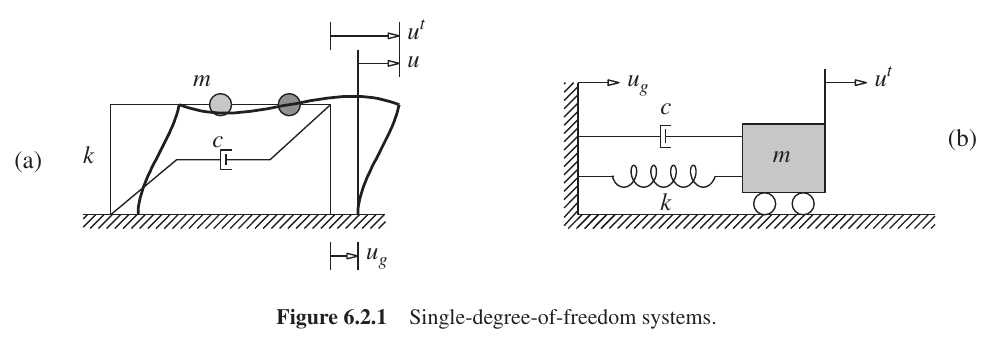
\includegraphics[width=.9\linewidth]{./figures/F6.2.1.png}
\end{center}
\end{itemize}
\item 6.3 反应量
\label{sec:org967a98d}
\begin{itemize}
\item 位移\(u(t)\) 、速度\(\dot{u}(t)\) 、加速度\(\ddot{u}(t)\)
\item 内力与位移线性相关:弯矩、剪力
\item 绝对位移\(u^{\mathrm{t}}(t)\) 确定相邻建筑留出间距防止碰撞
\item 绝对加速度\(\ddot{u}^{\mathrm{t}}(t)\) 确定传递给设备的运动
\end{itemize}
\item 6.4 反应时程
\label{sec:orgdc64c20}
\begin{itemize}
\item 图6.4.1ab比较了三个体系在El Centro地面加速度引起的位移反应
\item 用 \texttt{静力分析} 由 \(u(t)\) 中每个时刻的位移计算内力
\item 等效静力\(f_{\mathrm{s}}(t) = ku(t)\)
\item 用刚度 \(k\) 和 \(m\) 表示:\(f_{\mathrm{s}}(t) = m\omegann \ut\)
\item 其中角标 \(\mathrm{n}\) 表示的是自然之意
\item 引入 \texttt{伪加速度} \(A(t)\)
\item \(f_{\mathrm{s}}(t) = m\omega^{2}_{\mathrm{n}}u(t) = m A(t)\)
\item \(A(t) = \omega^{2}_{\mathrm{n}}u(t)\)
\item 由位移计算伪加速度
\item 由等效静力通过静力分析计算内力
\end{itemize}
\item 6.5 反应谱的概念
\label{sec:org19b5bc7}
\begin{itemize}
\item G. W. Housner 推动了反应谱的广泛应用
\item M. A. Biot 在1932年引入了这个概念
\item 反应谱
\begin{itemize}
\item 横轴是振动周期\(\Tn\) 或圆频率\(\omegann\) 或循环频率\(\fn\)
\item 纵轴是该周期或频率对应的反应量峰值(固定阻尼比\(\zeta\))
\item 位移反应谱 \(\uo \equiv \maxt \lvert u(t,T_{\mathrm{n},\zeta}) \rvert\)
\item 速度反应谱 \(\duo \equiv \maxt \lvert \dot{u}(t,T_{\mathrm{n},\zeta}) \rvert\)
\item 加速度反应谱 \(\dduo \equiv \maxt \lvert \ddot{u}^{\mathrm{t}}(t,T_{\mathrm{n},\zeta}) \rvert\)
\end{itemize}
\end{itemize}
\item 6.6 位移反应谱、伪速度反应谱和伪加速度反应谱
\label{sec:org2bbb07c}
\begin{itemize}
\item 6.6.1 位移反应谱
\label{sec:orga590f67}
\begin{itemize}
\item \(D \equiv u_{\mathrm{o}}\) 为峰值位移
\end{itemize}
\begin{center}
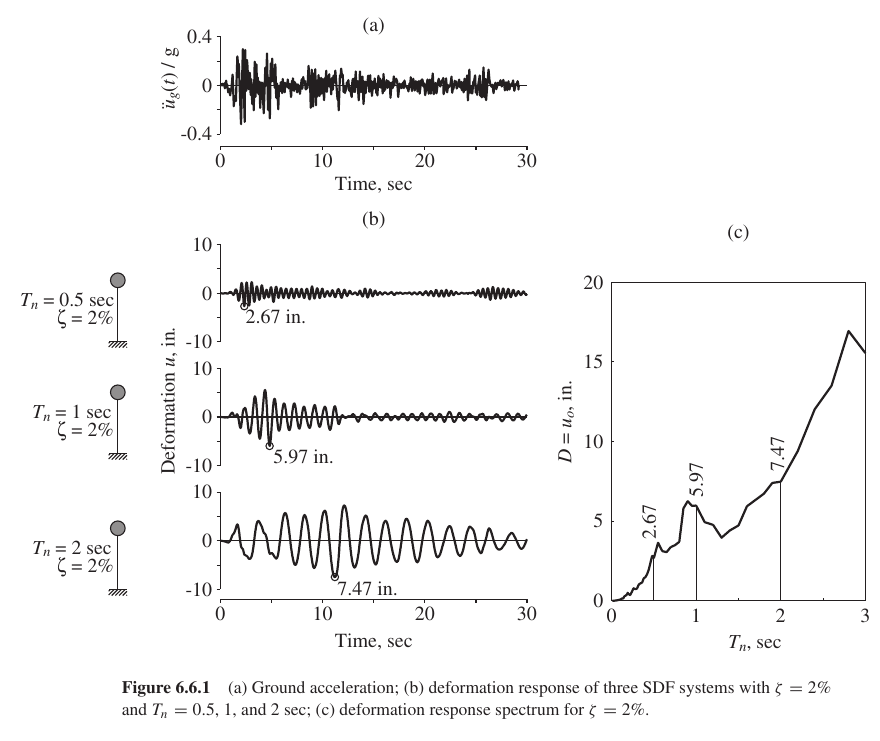
\includegraphics[width=.9\linewidth]{./figures/F6.6.1.png}
\end{center}
\item 6.6.2 伪速度反应谱
\label{sec:org90c21cf}
\begin{itemize}
\item \(V=\omega_{\mathrm{n}}D\)
\item 应变能 \(E_{\mathrm{S}_{\mathrm{o}}}=\dfrac{ku^{2}_{\mathrm{o}}}{2}=\dfrac{mV^{2}}{2}\)
\item \(V\) 峰值伪速度
\end{itemize}
\item 6.6.3 伪加速度反应谱
\label{sec:orgdbdaaf0}
\begin{itemize}
\item \(A=\omegann D\)
\item 峰值基底剪力 \(V_{\mathrm{bo}}=mA=\dfrac{A}{g}w\)
\item \(A/g\) \texttt{基底剪力系数} 或 \texttt{侧向力系数}
\item \(A\) 峰值伪加速度
\end{itemize}
\begin{center}
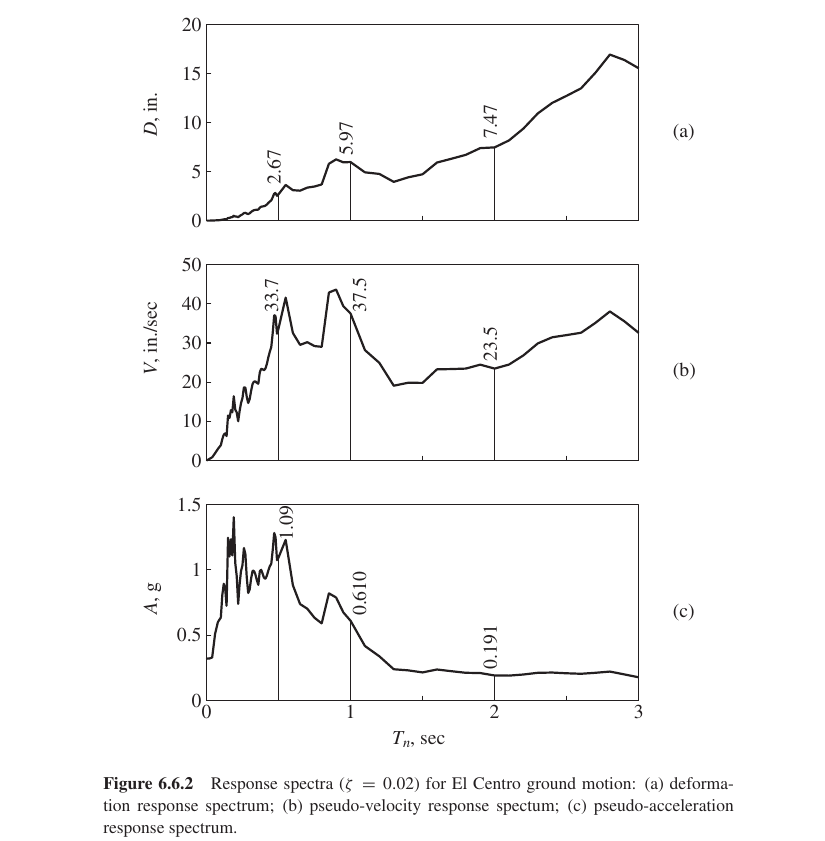
\includegraphics[width=.9\linewidth]{./figures/F6.6.2.png}
\end{center}
\item 6.6.4 D-V-A联合谱
\label{sec:org63510c4}
\begin{itemize}
\item A. S. Veletsos 和 N. M. Newmark 在1960年给出了联合形式的地震反应谱
\item 意义
\begin{enumerate}
\item 位移谱表示体系的峰值位移;伪速度谱表示峰值应变能;伪加速度与
等效静力及基底剪力相关
\item 由三个谱共同(而不是单独一个)近似估计设计谱的形式
\end{enumerate}
\end{itemize}
\item 6.6.5 反应谱的建立
\label{sec:orgc313e7a}
已知\(\ddot{u}_{\mathrm{g}}(t)\) ,按如下步骤建立反应谱
\begin{enumerate}
\item 数值定义\(\ddot{u}_{\mathrm{g}}(t)\) ,按时隔0.02秒
\item 选择\(T_{\mathrm{n}}\) 和\(\zeta\)
\item 数值方法求解\(u(t)\)
\item 确定峰值\(u_{\mathrm{o}}\)
\item 谱的纵坐标\(D\) 、\(V\) 、\(A\)
\item 在所有可能体系的\(T_{\mathrm{n}}\) 和\$\(\zeta\)\$中,重复第2到第5步
\item 制作反应谱
\end{enumerate}
\end{itemize}
\item 6.7 概据反应谱确定结构峰值反应
\label{sec:org07933e7}
\begin{itemize}
\item 例6.2 完整显示了线弹性单自由度体系的地震响应分析
\item 例6.3 说明了错误的优化方案。将结构设计得更刚带来了更大的惯性力,
伪加速度大了5倍;
\item 例6.4 一层钢混框架
\item 例6.5 倾斜地面建筑物
\item 例6.6 三跨箱形梁桥
\end{itemize}
\item 6.8 反应谱的特征
\label{sec:org5a68d4b}
\begin{itemize}
\item 分为三个谱区:位移敏感区(柔)、速度敏感区、加速度敏感区(刚)
\item 用正规的曲线拟合技术用选定形状的理想化反应谱代替实际值
\item 分隔谱区的周期、各段放大系数随地面运动的不同而不同、特别是峰值加
速度、速度和位移的相对值
\item 这些地需运动的特征取决于震级、断层距、震源、场地地质情况和场地条件
\end{itemize}
\item 6.9 弹性设计谱
\label{sec:org625cf59}
\begin{itemize}
\item 设计谱由一组光滑曲线或一系列直线组成,每条线对应一个阻尼水平
\item 均值反应谱
\item 均值加一个标准差反应谱
\item 绘制方法
\item 参数选择应基于震级、断层机理、地震波传播路径地质和局部场地进行
\item 峰值加速度设计值乘以设计谱值即可以得到场地设计谱
\end{itemize}
\item 6.10 设计谱与反应谱的比较
\label{sec:org3f323df}
\begin{itemize}
\item 图6.10.1显示标准设计谱与反应谱在加速度敏感区吻合较好,但在速度敏
感感区和位移敏感区差别很大
\item 图6.10.2显示差别依旧存在
\item 设计谱并不是为了与任何特定地面运动反应谱相吻合,而是使之能代表多
个地面运动的平均特征
\end{itemize}
\item 6.11 设计谱与反应谱之间的区别
\label{sec:orgbde4e03}
\begin{itemize}
\item 构造设计谱的方法是地震危险性分析的基础上得到的一致危险性谱
\end{itemize}
\item 6.12 速度反应谱和加速度反应谱
\label{sec:org99fcfef}
\begin{itemize}
\item 式(6.12.1)--(6.12.4)奠定了后面两个比较的逻辑基础
\end{itemize}
\begin{itemize}
\item 6.12.1 伪速度谱和相对速度谱
\label{sec:org493c5a0}
\begin{itemize}
\item 在长周期范围内,\(V\) 比\(\dot{u}_{\mathrm{o}}\) 明显较小,因为位
移有限,而\(T_{\mathrm{n}}\) 越大\(V\) 越小;而此时速度峰值趋近于
地面运动速度峰值
\item 在短周期内,比较(6.12.2)和(6.12.3)论证了二者相似的原因
\end{itemize}
\item 6.12.2 伪加速度谱和加速度谱
\label{sec:orgba75141}
\begin{itemize}
\item 无阻尼体系,由运动平衡方程即可看出二者是相同的
\item \(\dduto=-\omegann\ut\)
\item \(\dduto=\omegann \uo=\omegann D=A\)
\item 式(6.12.4)表明\(A\) 与\(\dduto\) 之间的差别会随阻尼的增加而增加
\item 在很长一段周期范围内,伪加速度都可以看作是真实加速度的近似
\end{itemize}
\end{itemize}
\end{itemize}
\subsection*{第7章 非弹性体系的地震反应}
\label{sec:orgab60274}
\subsection*{第8章 广义单自由度体系}
\label{sec:orgcab88fc}
\section*{第II篇 多自由度体系}
\label{sec:orgbe7cb2d}
\subsection*{第9章 运程方程、问题表述和求解方法}
\label{sec:orgd65d519}
\begin{itemize}
\item 9.1 简单体系:两层剪切型建筑
\label{sec:orgcbf578d}
\begin{itemize}
\item 9.1.1 使用牛顿第二运动定律
\label{sec:org5eb25c2}
\begin{itemize}
\item \(\vm \vddu + \vfd + \vfs = \vpt\)
\item \(\vm \vddu + \vc\vdu + \vk \vu = \vpt\)
\end{itemize}
\item 9.1.2 动平衡
\label{sec:org74172c8}
\begin{itemize}
\item D'Alembert原理
\end{itemize}
\item 9.1.3 质量-弹簧-阻尼器系统
\label{sec:org6721fe0}
\begin{itemize}
\item 经典两自由度体系由两个质量与线性弹簧和线性粘滞阻尼器组成
\end{itemize}
\item 9.1.4 刚度分量、阻尼分量和质量分量
\label{sec:org64577d0}
\begin{itemize}
\item 对于复杂体系运动方程的建立很有用
\end{itemize}
\end{itemize}
\item 9.2 线性体系的一般方法
\label{sec:orgaa46eba}
\begin{itemize}
\item 9.2.1 离散化
\label{sec:org2fa0158}
\item 9.2.2 弹性力
\label{sec:org82637e9}
\item 9.2.3 惯性力
\label{sec:orgaa9c3f0}
\item 9.2.4 阻尼力
\label{sec:orgf8edd3a}
\item 9.2.5 运动方程:外力
\label{sec:org8d5862b}
\end{itemize}
\item 9.3 静力凝聚
\label{sec:org58639a9}
\begin{itemize}
\item 静力凝聚法用来从动力分析中消除结构中那些具有零质量的自由度
\item 但所有自由度在静力分析中仍然是保留的
\item 凝聚刚度矩阵\(\vktta = \vktt - \vkott \vkoo^{-1} \vkot\)
\end{itemize}
\item 9.4 平面(或对称平面)体系:地面运动
\label{sec:org8ede222}
\item 9.5 单层平面非对称建筑物
\label{sec:org0a3f413}
\item 9.6 多层平面非对称建筑物
\label{sec:org9da16b8}
\item 9.7 多点支座激励
\label{sec:orgc9bfbcd}
\item 9.8 非弹性体系
\label{sec:org3c4e8ee}
\item 9.9 问题表述
\label{sec:org4b3a36f}
\item 9.10 单元力
\label{sec:org0a2d77e}
\item 9.11 运动方程的求解方法:概要
\label{sec:orgb401d44}
\end{itemize}
\subsection*{第10章 自由振动}
\label{sec:orgf1b9476}
\subsubsection*{第一部分:固有振动频率和振型}
\label{sec:org55d7d98}
\begin{itemize}
\item 10.1 无阻尼体系
\label{sec:orgda0573f}
\end{itemize}
\subsubsection*{第二部分:自由振动反应}
\label{sec:org747e749}
\subsubsection*{第三部分:振动特性的计算}
\label{sec:orgc2516fd}
\subsection*{第11章 结构中的阻尼}
\label{sec:orgbd375b3}
\subsection*{第12章 线性体系的动力分析和反应}
\label{sec:org940bf02}
\subsection*{第13章 线性体系的地震分析}
\label{sec:orgbfb5659}
\subsubsection*{第一部分:反应时程分析}
\label{sec:orgd5253ea}
\begin{itemize}
\item 13.1 振型分析
\label{sec:org3d0853e}
\begin{itemize}
\item 作用:地震引起的地面运动\(\ddugt\) 作用下结构反应
\item 方法:振型分析法
\item 假设:所有支撑点上的地面运动是相同的
\end{itemize}
\begin{itemize}
\item 13.1.1 运动方程
\label{sec:orgc9144a9}
\begin{itemize}
\item 运动方程:$$ \vm \vddu + \vc \vdu + \vk \vu = - \vm \viota  \ddugt $$
\item \quiz{所有质量都有受同样的加速度作用?} 参见式(9.4.9)
\item 地震反应分析中不需要考虑阻尼矩阵\(\vc\) ,振型阻比就足够了。
\end{itemize}
\item 13.1.2 位移和力的振型展开
\label{sec:org69a62ff}
\begin{itemize}
\item 位移展开:$$\vut = \sumn \vphin \qnt$$
\item 有效地震力的空间分布由\(\vs = \vm \viota\) 决定

\item 振型惯性力\(\vsn\) 之和的形式:
$$\vm\viota=\sumn \vsn = \sumn \Gamman \vm \vphin$$
其中:$$\Gamman = \dfrac{L_{n}}{M_{n}}, L_{n}=\vphint \vm \viota, M_{n}=\vphint \vm \vphin $$

\item 参与系数:\(\Gamman = \dfrac{\vphint \vm \viota }{\vphint \vm \vphin}\)
\item 第\(n\) 阶振型对\(\vm \viota\) 的贡献为:$$\vsn = \Gamman \vm \vphin$$
\item 力的振型展开向量:\(\vsn = \dfrac{\vphint \vm \viota \vm \vphin}{\vphint \vm \vphin}\)
\end{itemize}
\item 13.1.3 振型方程
\label{sec:org75ed0b3}
\begin{itemize}
\item 运动方程中荷载项为\(-\vm \viota \ddugt = - \sumn \vsn \ddugt\)
\item 考虑到力的振型展开,对于第\(n\) 阶振型,只考虑荷载 \(\vsn \ddugt = \Gamman \vm \vphin \ddugt\)
\item 按振型分析,第\(n\) 阶振型广义力为:\(\Pnt=\vphint \Gamman \vm \vphin \ddugt = \Gamman M_{n} \ddugt\)
\item 转化为标准型时荷载项即为:\(\dfrac{\Pnt}{M_{n}} = - \Gamman \ddugt\)
\item 方程(13.1.7)求解可以转化为方程(13.1.8)求解\(\Dn\) ,后\(\qnt=\Gamman \Dnt\)
\item 由 
\(\vm\viota=\sumn \vsn = \sumn \Gamman \vm \vphin\) 可知:$$\iota = \sumn \Gamman \vphin$$
\item \(\Gamman\) 称为振型参与系数。因与振型正则化方式有关,实际上并不采用
\item 振型贡献系数将用来用研究建筑物的地震效应
\end{itemize}
\item 13.1.4 振型反应
\label{sec:org920daf4}
\begin{itemize}
\item 位移 $$\vunt=\vphin \qnt = \Gamman \vphin \Dnt$$
\item 单元力用等效静力形式进行静力分析求解
\item 等效静力为 \(\vfnt = \vk \vunt\) ,代入\(\vk= \vm \omegann\) 及振型位移得:
$$\vfnt =  \vm \omegann \Gamman \vphin \Dnt = \vsn \omegann \Dnt = \vsn \Ant $$
\item 等效静力分为两部分:
\begin{itemize}
\item 将第\(n\) 阶振型对\(\vpefft\) 的空间分布\(\vm\viota\) 的贡献\(\vsn\)
\item 第\(n\) 阶振型单自由度体系在\(\ddugt\) 作用下的伪加速度反应
\end{itemize}
\item 第\(n\) 阶振型任意反应量\(\rt\) 的贡献\(\rnt\) 通过在\(\vfnt\) 作用下结构的静力分析确定
\item 定义\(\rnst\) 为\(\vsn\) 作用下\(r\) 的静力值,则有:\(\rnt = \rnst \Ant\)
\item 位移也可表达成上式
\begin{itemize}
\item 由\(\vk \vunst = \vsn\) 得:\(\vunst = \vk^{-1} \vsn = \vk^{-1} \Gamman \vm \vphin\)
\item 由\(\vk^{-1}\vm = \dfrac{1}{\omegann}\) ,有\(\vunst = \dfrac{\Gamman}{\omegann}\vphin\)
\begin{itemize}
\item 则:\(\vunt = \dfrac{\Gamman}{\omegann} \vphin \Ant\)
\end{itemize}
\end{itemize}
\end{itemize}
\item 13.1.5 总反应
\label{sec:orge0021ef}
\begin{itemize}
\item 位移:\(\vut = \sumn \vunt =  \sumn \Gamman \vphin \Dnt\)
\item 反应:\(\rt = \sumn \rnt = \sumn \rnst \Ant\)
\end{itemize}
\item 13.1.6 振型分析的解释
\label{sec:org6931e7d}
\begin{itemize}
\item 步骤
\begin{enumerate}
\item 计算结构的振动特性(固有频率和振型)
\item 将力分布向量\(\vm\viota\) 展开成其振型分量\(\vsn\)
\item 做\(N\) 组振型分析
\begin{itemize}
\item 在\(\vsn\) 作用下做结构静力分析\(\rnst\)
\item 在\(\ddugt\) 作用下第\(n\) 阶单自由度体系的动力分析\(\Ant\)
\item 振型分析响应\(\rnt=\rnst \Ant\)
\end{itemize}
\end{enumerate}
\item E13.1展示了完整的地震反应时程分析
\end{itemize}
\item 13.1.7 对基础转动的反应分析
\label{sec:orga443907}
\begin{itemize}
\item \(\vpefft= - \vm \viota \ddthetagt\)
\item \(\viota\) 为由单位基础转动\(\theta_{\mahtm{g}} =1\) 引起的所有自由度的静力位移向量
\end{itemize}
\end{itemize}
\item 13.2 具有对称平面的多层建筑物
\label{sec:org4e96973}
\begin{itemize}
\item 将13.1节的振型分析法分析多层建筑物
\item 运动方程 $$ \vm \vddu + \vc \vdu + \vk \vu = - \vm \unity \ddugt  $$
\item 其中:
\begin{itemize}
\item \(\unity\) 是每个元素均为1的向量;
\item \(\vm\) 是\(m_{jj}=m_{j}\) 的对角矩阵;
\item 对照此前的线性体系运动方程,影响向量\(\viota = \unity\)
\end{itemize}
\end{itemize}
\begin{itemize}
\item 13.2.1 有效地震力的振型展开
\label{sec:orgca51aa6}
\begin{itemize}
\item 由于\(\vm\) 为对角矩阵,可以书写中简化为(13.2.3)形式
$$\vm \unity = \sumn \vsn = \sumn \Gamman \vm \vphin$$
\item 其中:\(\Gamman = \dfrac{\Lnh}{M_{n}}\) ,\(\Lnh=\sumn m_{j}\phi_{jn}\) ,\(M_{n}=\sumn m_{j}\phi^{2}_{jn}\)
\item 这里没有说明为什么标记\(\Lnh\)
\item \(\vsn = \Gamman \vm \vphin\) ,\(s_{jn} = \Gamman m_{j} \phi_{jn}\)
\item E13.2演示了空间分布\(\vm \unity\) 的振型展开
\end{itemize}
\item 13.2.2 振型反应
\label{sec:orgdaf5229}
\begin{itemize}
\item 定义了\(\Mns\) 和\(\Lns\) 不知道是意义何在,译者应说明在节13.2.5中给出解释
\end{itemize}
\item 13.2.3 总反应
\label{sec:orgad9bfc3}
\begin{itemize}
\item 式(13.2.11)用来计算楼层加速度,但加速度用来干嘛呢
\end{itemize}
\item 13.2.4 小结
\label{sec:orgaec845f}
\begin{itemize}
\item 基本同此前的振型分析,只是振型分量\(\vsn\) 表达稍简化
\end{itemize}
\item 13.2.5 有效振型质量和有效振型高度
\label{sec:org3a03297}
\begin{itemize}
\item \(M^{*}_{n}\) 称为基底剪力有效振型质量,或有效振型质量
\item \(h^{*}_{n}\) 称为基底力矩有效振型高度,或有效振型高度
\end{itemize}
\item 13.2.6 例题:五层剪切型框架
\label{sec:org89492fb}
\item 13.2.7 带附属结构的四层框架
\label{sec:org23ef511}
\end{itemize}
\item 13.3 具有非对称平面的多层建筑物
\label{sec:orgf6cf087}
\item 13.4 平面对称多层建筑物的扭转反应
\label{sec:org082ea6c}
\item 13.5 对多点支座激励的反应分析
\label{sec:org6f96c4c}
\item 13.6 结构的理想化与地震反应
\label{sec:org8afa940}
\end{itemize}
\subsubsection*{第二部分:反应谱分析}
\label{sec:org6b0c17b}
\begin{itemize}
\item 13.7 根据地震反应谱求峰值反应
\label{sec:orgc4ff4c3}
\begin{itemize}
\item 结构设计通常基于地震引起的反应持续时段内内力和变形的峰值
\item 多分量同时作用及多支点支座扰动的RSA应该关注
\end{itemize}
\begin{itemize}
\item 13.7.1 峰值振型反应
\label{sec:org64954d1}
\begin{itemize}
\item \(\rno\) 与第6章 \(\uo\) 中的角标\(\mathrm{o}\) 不同,前者表示带符号的峰值,后者表示绝对值最大值
\end{itemize}
\item 13.7.2 振型组合规则
\label{sec:org20f48f3}
\begin{itemize}
\item 各振型的峰值并不是同时达到的,这就会产生一个问题:怎样组合峰值
振型反应\(\rno\) 来确定总反应的峰值\(\ro \equiv \maxt \lvert \rt \rvert\)
\item 绝对相加ABSSUM,\(\ro \leqslant \sumn \lert \rt \vert\) 过于保守,实用中并不普遍
\item SRSS: \(\ro \cong \left( \sumn \ro^{2} \right) ^{1/2}\)
\item 什么是稀疏固定频谱结构
\item CQC:\(\ro \cong \left( \sumn \sumn \rhio \rio \rno \right) ^{1/2}\)
\item CQC展开:\(\ro \cong \left( \sumn \rno^{2} + \sumin \rhio \rio \rno \right) ^{1/2}\)
\item 图13.7.1显示了两类CQC规则的差异
\item 并在稍后解释了SRSS规则局限性的原因
\item 对于小阻尼结构,频比在1.3以上时,相关系数基本为零
\end{itemize}
\item 13.7.3 反应谱分析的解释
\label{sec:org63592d7}
\begin{itemize}
\item RSA是地震激励作用下结构动力分析的一种方法,但简化为静力分析
\item 通过\(\vsn\) 作用下结构的静力分析得到振型静力反应\(\rnst\)
\item 再乘以反应谱纵坐标\(\An\) 得到峰值振型反应\(\rno\)
\item RSA方法仍然是一种动力分析方法,因为它利用了结构的振动特性和用
反应谱(设计谱)所表征的地面运动的动力特性
\end{itemize}
\end{itemize}
\item 13.8 具有对称平面多层建筑物
\label{sec:org4b82aa6}
\begin{itemize}
\item 
\end{itemize}
\item 13.9 具有非对称平面多层建筑物
\label{sec:org48291cc}
\item 13.10 基于反应谱的同步反应包络
\label{sec:orgf40de6c}
\item 13.11 多分量地面运动作用下的峰值反应
\label{sec:org3bae673}
\end{itemize}
\subsection*{第14章 非经典阻尼体系的分析}
\label{sec:org003d593}
\subsection*{第15章 自由度的缩减}
\label{sec:orgdec7f81}
\subsection*{第16章 动力反应的数值计算}
\label{sec:orgc3804cf}
\subsection*{第17章 具有分布质量和弹性体系}
\label{sec:org87cd1d3}
\subsection*{第18章 有限单元法初步}
\label{sec:orge0a4350}
\section*{第III篇 多层建筑地震响应、设计与评估}
\label{sec:orgf9517f8}
\subsection*{第19章 线弹性建筑物的地震反应}
\label{sec:org5e50fc4}
\begin{itemize}
\item 19.1 所分析的体系、设计谱和反应量
\label{sec:org509d21d}
\begin{itemize}
\item 19.1.1 所分析的体系
\label{sec:org4cdc3a0}
\begin{itemize}
\item 引入梁柱(刚度)比\(\rho\) 概念
\item 图19.1.3显示了刚度比\(\rho\) 对基频的影响。\(\rho\) 越大,基频越大。
\item 图19.1.4说明了\(\rho\) 对周期分离程度比的影响,\(\rho\) 越大,各阶频率越接近
\end{itemize}
\item 19.1.2 设计谱
\label{sec:orgc2477b6}
\begin{itemize}
\item 图19.1.6再次说明了谱分区要靠D-V-A合谱确定
\item 通过伪加速度比例,即可知峰值加速度对应的谱
\end{itemize}
\item 19.1.3 设计谱
\label{sec:orgf5342f4}
\begin{itemize}
\item \(W^{*}_{1}\) 和\(h^{*}_{1}}\) 依赖于\(\rho\)
\end{itemize}
\end{itemize}
\item 19.1.3 \(T_{1}\) 和\(\rho\) 对反应的影响
\label{sec:orga7935d9}

\item 19.1.4 振型贡献系数
\label{sec:org54273e6}
\item 19.1.4 \(T_{1}\) 对高阶振型反应的影响
\label{sec:org6dd3eea}
\end{itemize}

\subsection*{第20章 非弹性建筑物的地震反应分析与反应}
\label{sec:org00b99d4}
\subsection*{第21章 基底隔震建筑物地的地震动力学}
\label{sec:org47dd016}
\subsection*{第22章 建筑规范中的结构动力学}
\label{sec:org10c2e96}
\subsection*{第23章 建筑物的评估标准中的结构动力学}
\label{sec:org18c589c}
\end{document}